\documentclass[aspectratio=169]{beamer}

\usepackage[utf8]{inputenc}
\usepackage{graphicx}
\usepackage{tikz}
\usetikzlibrary{positioning, arrows.meta, shapes.symbols}
\usepackage{pifont}

\usefonttheme{professionalfonts}

% Theme
\usetheme{Madrid}
\definecolor{ucdgreen}{RGB}{0, 102, 51}
\definecolor{gapred}{RGB}{180, 50, 50}
\definecolor{stepfill}{RGB}{230, 243, 235}
\definecolor{topfill}{RGB}{0, 102, 51}
\definecolor{donefill}{RGB}{200, 230, 210}
\definecolor{nextfill}{RGB}{255, 240, 200}
\usecolortheme[named=ucdgreen]{structure}
\setbeamertemplate{navigation symbols}{}

\title[Research Studies Panel]{Research Studies Panel}
\author[Lainey Ward]{Lainey Ward}
\institute[]{Decarb-AI Centre, School of Civil Engineering\\
Primary supervisor: Dr Fiachra O'Loughlin \\ Co-supervisor: Dr Conor Sweeney}
\date{}

\begin{document}

% --------------------------------------------------
% SLIDE 0: Title page
% --------------------------------------------------
% PURPOSE: Greeting, intro for Abdollah, three-part overview.
%          All spoken — slide just shows name, centre, supervisors.
% --------------------------------------------------
\begin{frame}
    \titlepage
\end{frame}

% --------------------------------------------------
% SLIDE 1: The S2S timescale + what this thesis targets
% --------------------------------------------------
% PURPOSE: Establish what S2S is and introduce drought-to-flood
%          transitions as the target phenomenon. Script carries
%          the multi-hazard explanation verbally.
% --------------------------------------------------
\begin{frame}{What Is the Prediction Gap?}

    \begin{columns}[c, totalwidth=\textwidth]

        % ── Left: Mariotti figure ─────────────────────────
        \begin{column}{0.72\textwidth}
            \centering
            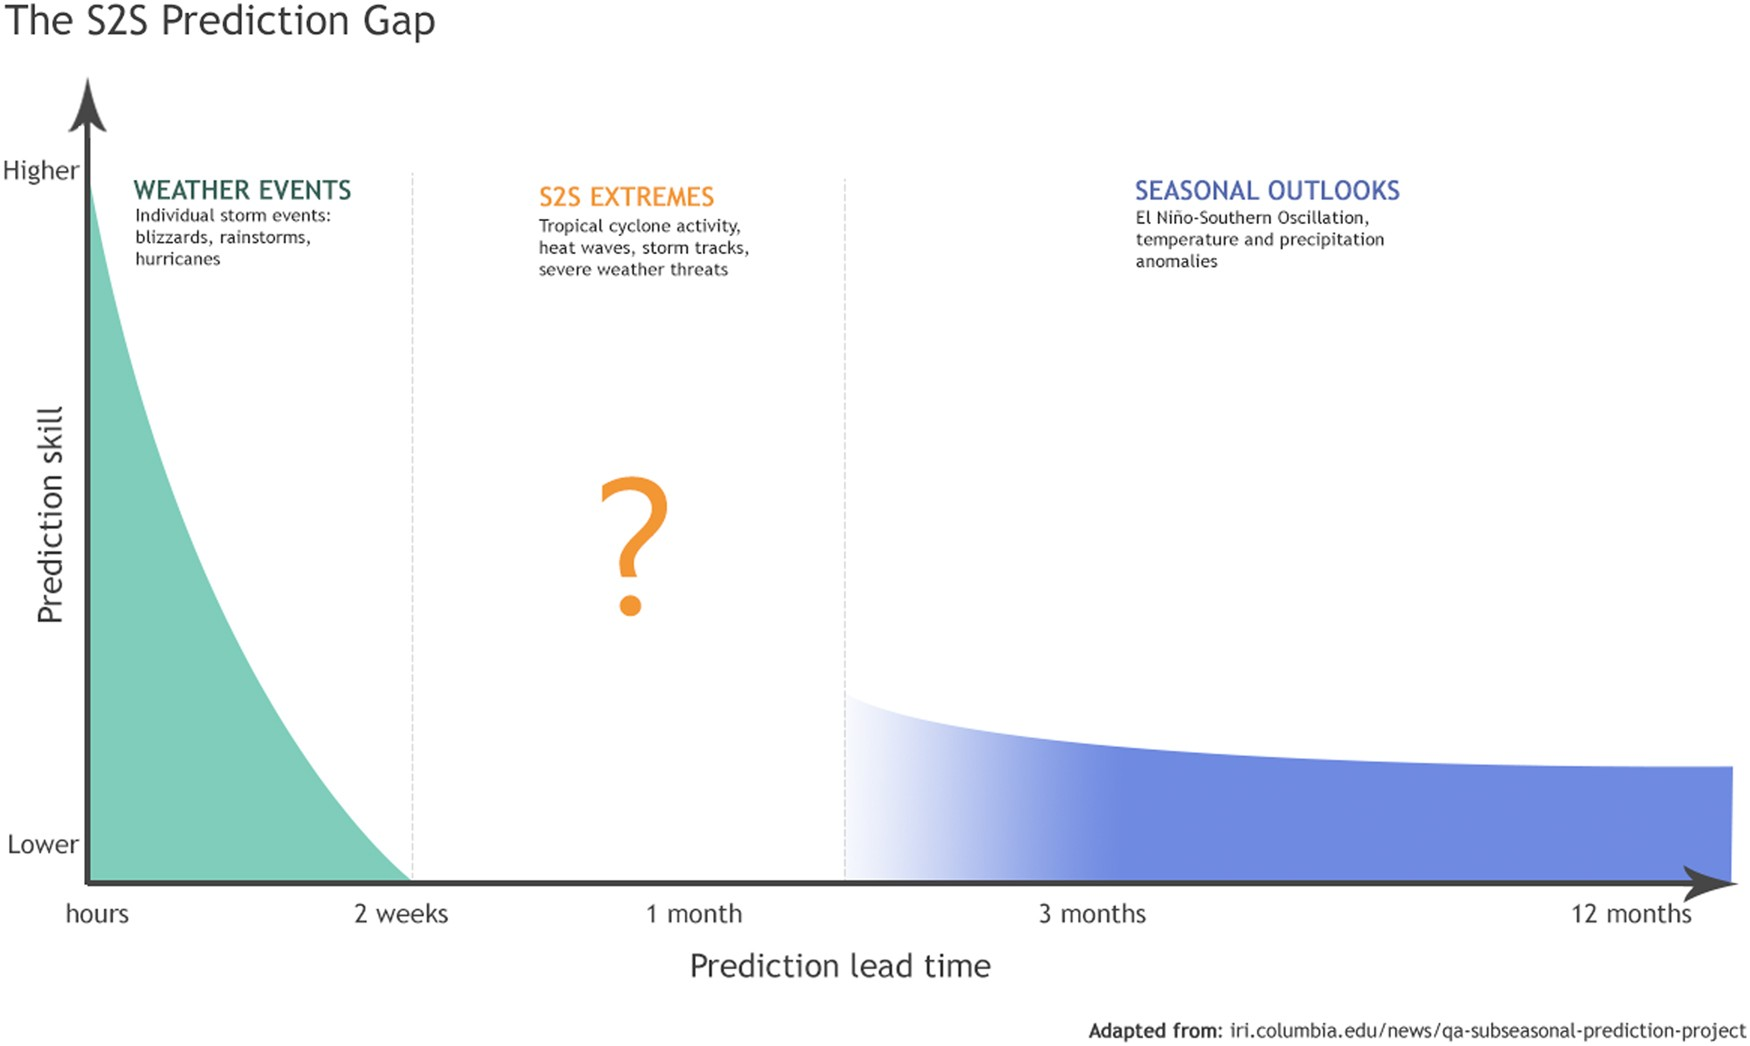
\includegraphics[width=\textwidth, keepaspectratio,
                trim=0 30 0 0, clip]
                {s2s_prediction_gap_mariotti2018.jpg}\\[-0.2em]
            {\tiny\color{gray!50} Source: Mariotti et al.\ (2018)}
        \end{column}

        % ── Right: 24% stat ──────────────────────────────
        \begin{column}{0.26\textwidth}
            \centering
            \vspace{1cm}
            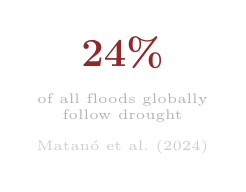
\begin{tikzpicture}
                \node[font=\Large\bfseries, text=gapred!80!black]
                    at (0, 0) {24\%};
                \node[font=\tiny, text=gray!60, align=center]
                    at (0, -0.7) {of all floods globally\\follow drought};
                \node[font=\tiny, text=gray!40]
                    at (0, -1.2) {Matan\'o et al.\ (2024)};
            \end{tikzpicture}
        \end{column}

    \end{columns}

\end{frame}

% --------------------------------------------------
% SLIDE 2: Literature review findings + staircase
% --------------------------------------------------
% PURPOSE: Show what the literature does (three levels),
%          where it stops (Level 3), and what must be built
%          to get there (staircase of contributions).
% --------------------------------------------------
\begin{frame}{What Does the Literature Say?}

    \centering
    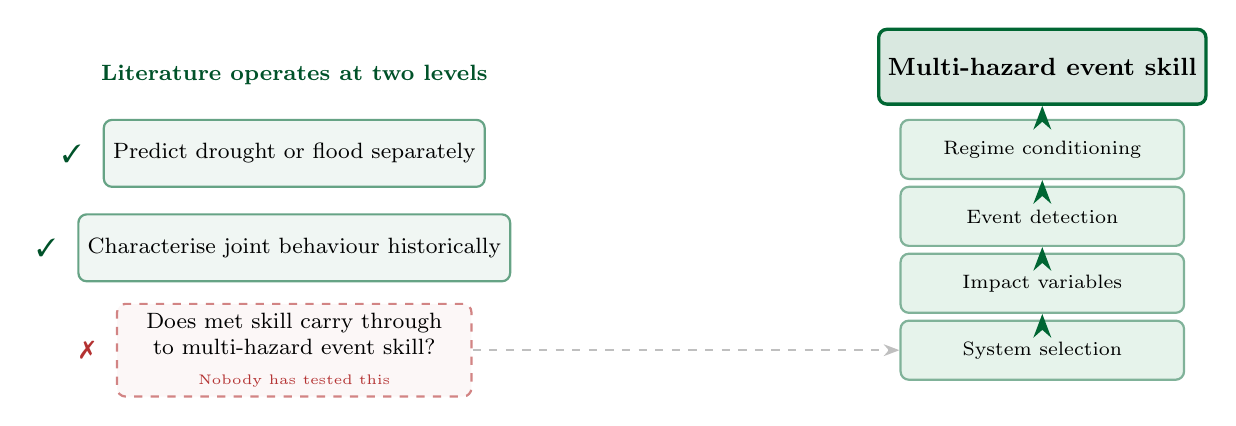
\begin{tikzpicture}[
        % Styles
        level/.style={
            draw=ucdgreen!60, thick, rounded corners=3pt,
            minimum width=4.8cm, minimum height=0.85cm,
            fill=ucdgreen!6, align=center, font=\footnotesize
        },
        levelgap/.style={
            draw=gapred!60, thick, rounded corners=3pt, dashed,
            minimum width=4.8cm, minimum height=0.85cm,
            fill=gapred!4, align=center, font=\footnotesize
        },
        stair/.style={
            draw=ucdgreen!50, thick, rounded corners=3pt,
            minimum width=3.6cm, minimum height=0.75cm,
            fill=stepfill, align=center, font=\scriptsize
        },
        topstair/.style={
            draw=ucdgreen, very thick, rounded corners=3pt,
            minimum width=3.6cm, minimum height=0.75cm,
            fill=topfill!15, align=center, font=\scriptsize\bfseries
        },
        tick/.style={font=\small, text=ucdgreen!80!black},
        cross/.style={font=\small, text=gapred},
        arr/.style={-{Stealth[length=2mm]}, thick, gray!50}
    ]

    % === LEFT: Three levels ===
    \node[font=\footnotesize\bfseries, text=ucdgreen!80!black]
        at (-5.0, 2.8) {Literature operates at two levels};

    % Level 1
    \node[level, minimum width=4.5cm] (l1) at (-5.0, 1.8)
        {Predict drought or flood separately};
    \node[tick, left=0.15cm of l1] {\ding{51}};

    % Level 2
    \node[level, minimum width=4.5cm] (l2) at (-5.0, 0.6)
        {Characterise joint behaviour historically};
    \node[tick, left=0.15cm of l2] {\ding{51}};

    % Level 3 — the gap
    \node[levelgap, minimum width=4.5cm, minimum height=1.1cm] (l3) at (-5.0, -0.7)
        {Does met skill carry through\\to multi-hazard event skill?\\[0.15em]
         {\tiny\color{gapred} Nobody has tested this}};
    \node[cross, left=0.15cm of l3] {\ding{55}};

    % === RIGHT: Staircase ===
    \node[font=\footnotesize\bfseries, text=ucdgreen!80!black]
        at (4.5, 2.8) {What must be built};

    % Step 1: System selection
    \node[stair] (s1) at (4.5, -0.7)
        {System selection};

    % Connector from Level 3 to staircase
    \draw[-{Stealth[length=2mm]}, thick, gray!50, dashed]
        (l3.east) -- (s1.west);

    % Step 2: Impact variables
    \node[stair] (s2) at (4.5, 0.15)
        {Impact variables};
    \draw[-{Stealth[length=3mm]}, very thick, ucdgreen]
        (s1.north) -- (s2.south);

    % Step 3: Event detection
    \node[stair] (s3) at (4.5, 1.0)
        {Event detection};
    \draw[-{Stealth[length=3mm]}, very thick, ucdgreen]
        (s2.north) -- (s3.south);

    % Step 4: Regime conditioning
    \node[stair] (s4) at (4.5, 1.85)
        {Regime conditioning};
    \draw[-{Stealth[length=3mm]}, very thick, ucdgreen]
        (s3.north) -- (s4.south);

    % Top: Event skill
    \node[topstair, minimum height=0.95cm, minimum width=4.0cm,
          font=\small\bfseries] (s5) at (4.5, 2.9)
        {Multi-hazard event skill};
    \draw[-{Stealth[length=3mm]}, very thick, ucdgreen]
        (s4.north) -- (s5.south);

    \end{tikzpicture}

\end{frame}

% --------------------------------------------------
% SLIDE 3: Research Questions + Three Papers + Paper 1 Roadmap
% --------------------------------------------------
% PURPOSE: State the two research questions, introduce the three
%          papers, and show the Paper 1 roadmap. Script says
%          "The roadmap on screen shows how Paper 1 maps out."
% --------------------------------------------------
\begin{frame}{Research Arc}

    % --- Two research questions ---
    \vspace{0.3em}
    \begin{enumerate}
        \item[\textcolor{ucdgreen}{\textbf{1.}}] {\itshape How does prediction skill at S2S lead times compare across forecast variables, impact variables, and multi-hazard events?}
        \item[\textcolor{ucdgreen}{\textbf{2.}}] {\itshape Under what atmospheric conditions does this skill emerge?}
    \end{enumerate}

    \vspace{0.6em}

    % --- Three papers ---
    \centering
    
\begin{tikzpicture}[
        pbox/.style={draw=ucdgreen!40, thick, rounded corners=4pt,
            minimum width=4.0cm, minimum height=1.2cm,
            fill=ucdgreen!5, align=center, font=\footnotesize}
    ]
    \node[pbox, fill=donefill, draw=ucdgreen!60] (pa) at (0, 0)
        {\textbf{Paper 1}\\[0.15em]
         {\scriptsize Drought-to-flood}\\[-0.1em]
         {\tiny\color{ucdgreen!70!black} temporally compounding}};
    \node[pbox, fill=nextfill, draw=orange!50] (pb) at (4.8, 0)
        {\textbf{Paper 2}\\[0.15em]
         {\scriptsize RES droughts}\\[-0.1em]
         {\tiny\color{orange!70!black} multivariate}};
    \node[pbox, fill=gray!8, draw=gray!40] (pc) at (9.6, 0)
        {\textbf{Paper 3}\\[0.15em]
         {\scriptsize ANTICIPATE COST Action}\\[-0.1em]
         {\tiny\color{gray} to be determined}};
    \end{tikzpicture}

    \vspace{1.2em}

    % --- Paper 1 roadmap (chevron chain) ---
    \centering
    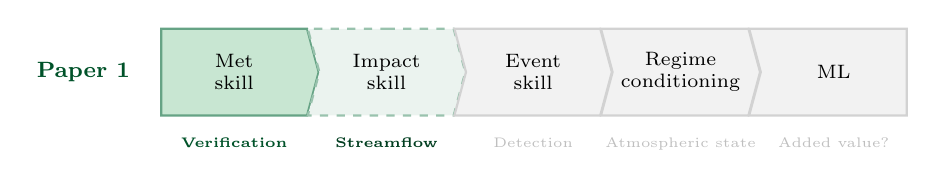
\begin{tikzpicture}[
        xscale=1.0,
        chev/.style={
            minimum width=2.0cm, minimum height=1.1cm,
            align=center, font=\scriptsize, inner sep=3pt,
            signal, signal to=east, signal from=west,
            signal pointer angle=150,
            thick
        },
        plbl/.style={font=\tiny, below=0.15cm}
    ]

    % Label
    \node[font=\footnotesize\bfseries, text=ucdgreen!80!black,
          anchor=east] at (-1.2, 0) {Paper 1};

    % Met skill — near complete (green)
    \node[chev, fill=donefill, draw=ucdgreen!60,
          signal from=none] (p1) at (0, 0)
        {Met\\skill};
    \node[plbl, text=ucdgreen!80!black, font=\tiny\bfseries]
        at (p1.south) {Verification};

    % Impact skill — next (light green, not amber)
    \node[chev, fill=ucdgreen!8, draw=ucdgreen!40, dashed,
          right=-0.02cm of p1] (p2)
        {Impact\\skill};
    \node[plbl, text=ucdgreen!60!black, font=\tiny\bfseries]
        at (p2.south) {Streamflow};

    % Event skill — planned (grey)
    \node[chev, fill=gray!10, draw=gray!35,
          right=-0.02cm of p2] (p3)
        {Event\\skill};
    \node[plbl, text=gray!50]
        at (p3.south) {Detection};

    % Regime conditioning — planned (grey)
    \node[chev, fill=gray!10, draw=gray!35,
          right=-0.02cm of p3] (p4)
        {Regime\\conditioning};
    \node[plbl, text=gray!50]
        at (p4.south) {Atmospheric state};

    % ML — planned (grey)
    \node[chev, fill=gray!10, draw=gray!35,
          signal to=none, right=-0.02cm of p4] (p6)
        {ML};
    \node[plbl, text=gray!50]
        at (p6.south) {Added value?};

    \end{tikzpicture}

\end{frame}

\end{document}
